\chapter{Niveles Sonoros Relevados}
\label{sec:mediciones}

\section{Registro de Datos Temporales Exportados}
Durante la sesión de ensayo de $306,69\s$, la aplicación Sound Analyzer registró 3302 muestras temporales. En la
Tabla~\ref{tab.ej1:mediciones} se presentan los niveles sonoros instantáneos $L_{AF}$ y equivalentes acumulados
$L_{Aeq}$ extraídos en intervalos representativos de $30\s$.

\begin{table}[!ht]
  \centering
  \caption{Evolución temporal del nivel sonoro instantáneo $L_{AF}$ y equivalente $L_{Aeq}$.}
  \label{tab.ej1:mediciones}
    \begin{tabular}{ccc}
      \toprule
      \textbf{Tiempo $t$ [\text{s}]} & \textbf{$L_{AF}$ [\text{dBA}]} & \textbf{$L_{Aeq}$ [\text{dBA}]} \\
      \midrule
      0,1 & 66,2 & 68,0 \\
      30,0 & 83,1 & 83,8 \\
      60,0 & 86,2 & 84,4 \\
      90,0 & 87,6 & 84,7 \\
      120,0 & 86,3 & 84,9 \\
      150,0 & 86,5 & 85,0 \\
      180,0 & 86,1 & 85,0 \\
      210,0 & 85,1 & 84,9 \\
      240,0 & 85,5 & 84,8 \\
      270,0 & 85,3 & 84,7 \\
      306,7 & 65,5 & 84,66 \\
      \bottomrule
    \end{tabular}%
\end{table}

\section{Valores Característicos Registrados}
Los parámetros estadísticos globales obtenidos al finalizar el procesamiento continuo del archivo de mediciones se
resumen en la Tabla~\ref{tab.ej1:resumen_valores}.

\begin{table}[!ht]
  \centering
  \caption{Resumen de parámetros sonoros característicos del ensayo.}
  \label{tab.ej1:resumen_valores}
    \begin{tabular}{lc}
      \toprule
      \textbf{Parámetro Acústico} & \textbf{Valor Medido} \\
      \midrule
      Nivel Sonoro Mínimo Instantáneo ($L_{AF,min}$) & $55,71\dBA$ \\
      Nivel Sonoro Máximo Instantáneo ($L_{AF,max}$) & $89,22\dBA$ \\
      Nivel Sonoro Continuo Equivalente Final ($L_{Aeq,final}$) & $84,66\dBA$ \\
      Nivel Sonoro Pico Ponderado C ($L_{CF,max}$) & $91,57\dBC$ \\
      Duración Total de Muestreo ($T_{muestra}$) & $306,69\s$ ($5\text{ min } 6\text{ s}$) \\
      \bottomrule
    \end{tabular}%
\end{table}

\section{Visualización de Resultados y Gráficos Temporales}
La Figura~\ref{fig.ej1:screenshot_app} exhibe la pantalla final de la aplicación Sound Analyzer al concluir la adquisición,
confirmando los valores estables de $L_{AF,max} = 89,22\dBA$ y $L_{Aeq} = 84,66\dBA$.

\begin{figure}[!ht]
  \centering
  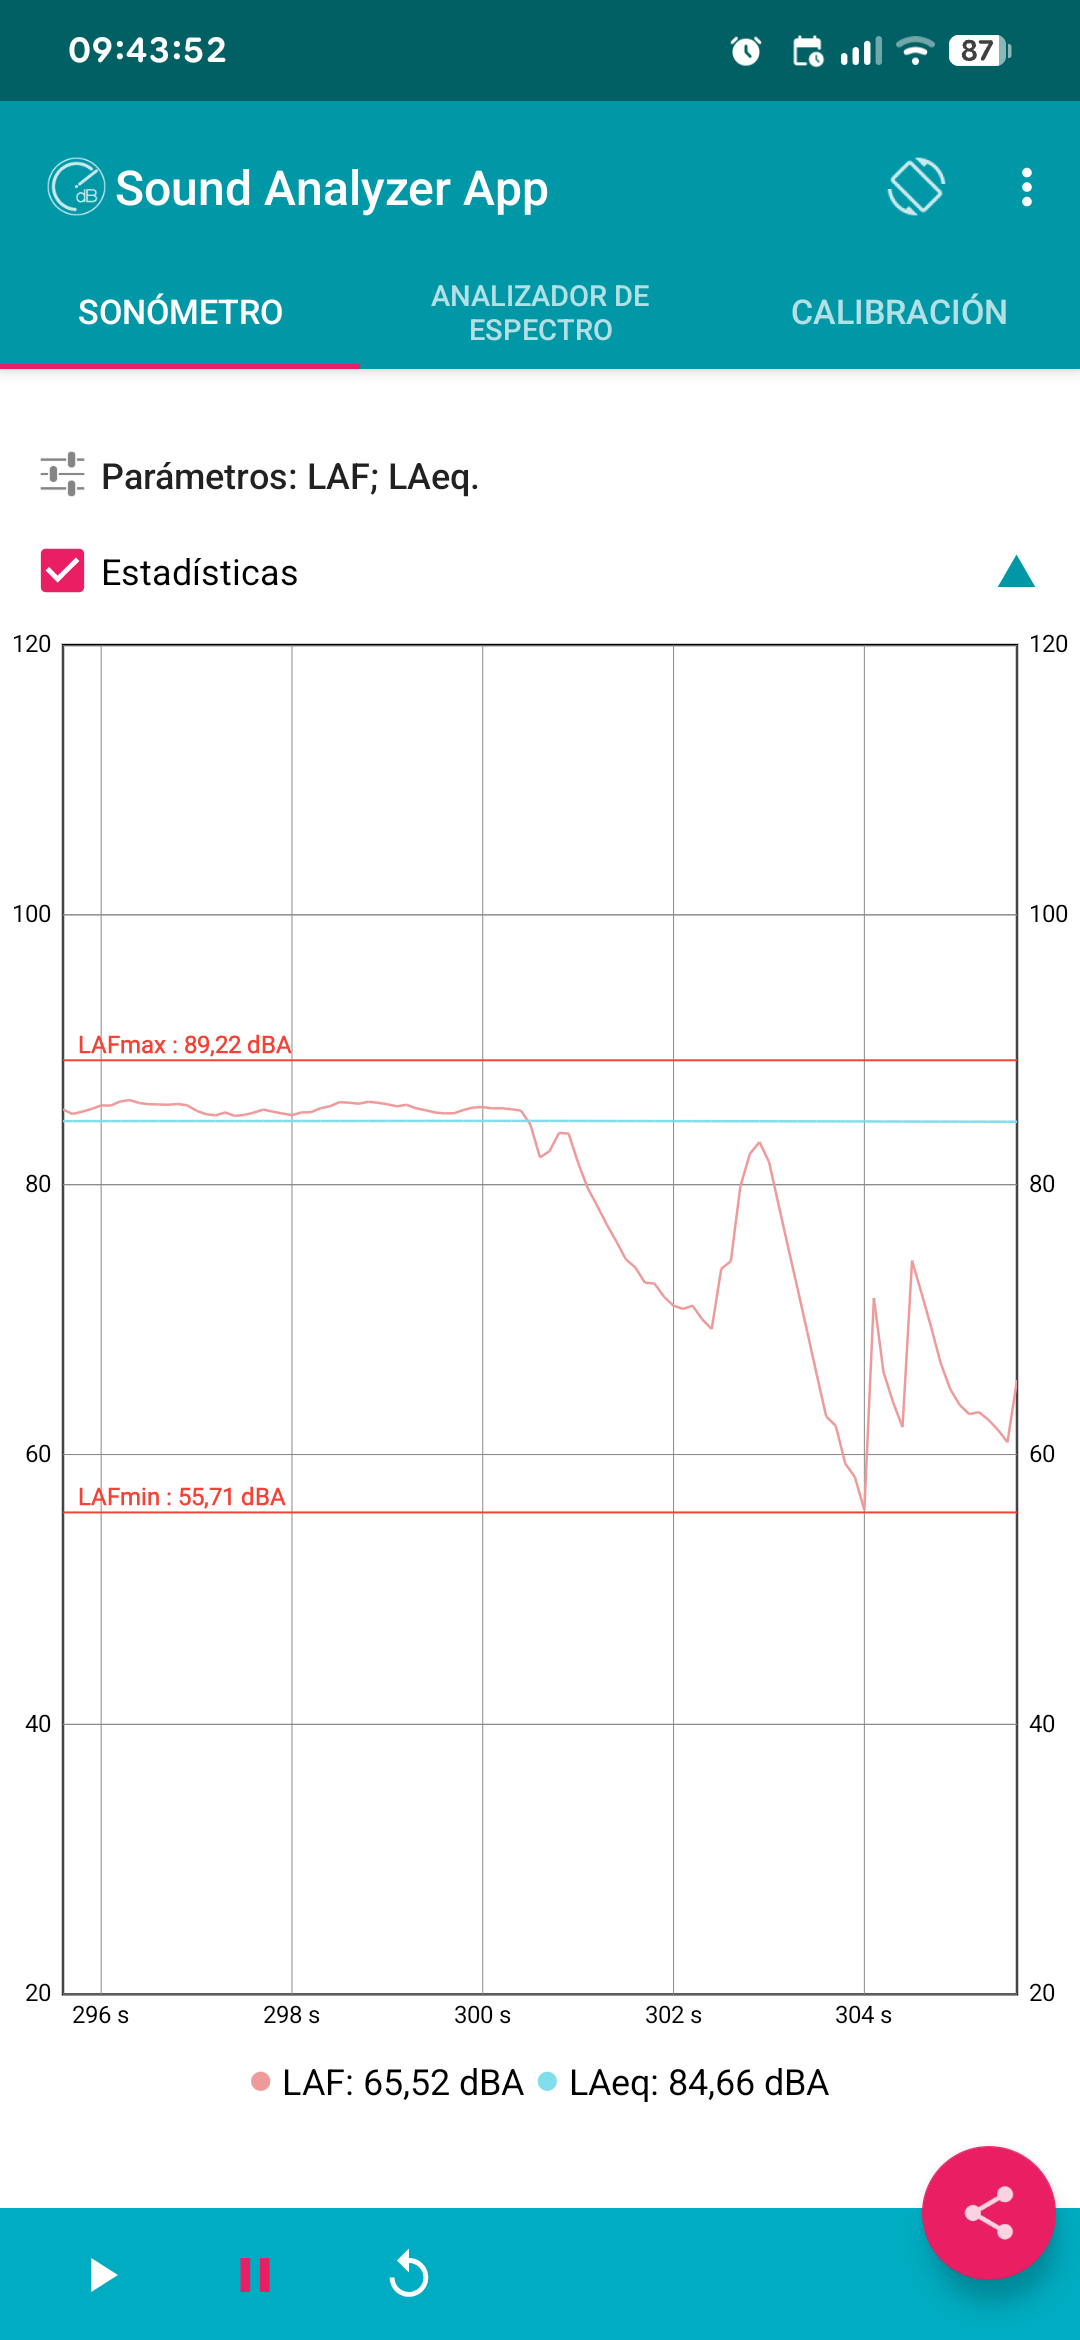
\includegraphics[width=0.45\textwidth]{images/screenshot_sound_analyzer.png}
  \caption{Captura de pantalla final de la aplicación Sound Analyzer v2.7 al concluir el ensayo.}
  \label{fig.ej1:screenshot_app}
\end{figure}

Por su parte, en la Figura~\ref{fig.ej1:evolucion_ruido} se representa la totalidad de las variaciones del nivel sonoro
$L_{AF}$ junto con el proceso de convergencia del $L_{Aeq}$ y el límite legal de $85\dBA$. En el gráfico se observan
claramente las caídas periódicas de presión sonora correspondientes a los pausas de $5\s$ entre ciclos de trabajo.

\begin{figure}[!ht]
  \centering
  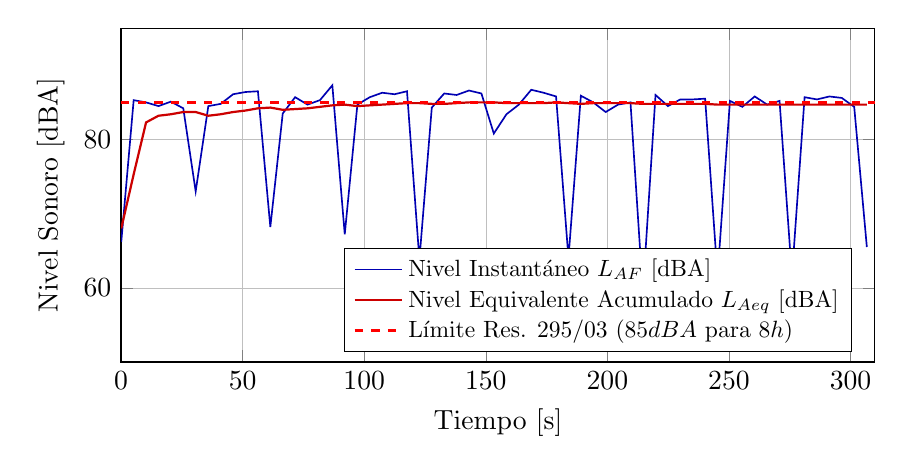
\begin{tikzpicture}
  \begin{axis}[
    width=0.92\textwidth,
    height=0.48\textwidth,
    xlabel={Tiempo [\text{s}]},
    ylabel={Nivel Sonoro [\text{dBA}]},
    xmin=0, xmax=310,
    ymin=50, ymax=95,
    grid=both,
    grid style={line width=.1pt, draw=gray!20},
    major grid style={line width=.2pt, draw=gray!50},
    legend pos=south east,
    legend cell align={left},
    legend style={nodes={scale=0.85, transform shape}}
  ]

    % Curva de LAF (Mediciones reales TSV Sound Analyzer App)
    \addplot[
      color=blue!70!black,
      semithick,
      mark=none
    ] coordinates {
      (0.1,66.2) (5.2,85.3) (10.3,85.0) (15.4,84.5) (20.5,85.1) (25.6,84.2)
      (30.7,73.0) (35.9,84.5) (41.0,84.8) (46.1,86.1) (51.2,86.4) (56.3,86.5)
      (61.4,68.2) (66.5,83.5) (71.6,85.7) (76.7,84.7) (81.8,85.3) (86.9,87.3)
      (92.0,67.2) (97.2,84.7) (102.3,85.7) (107.4,86.3) (112.5,86.1) (117.6,86.5)
      (122.7,63.8) (127.8,84.3) (132.9,86.2) (138.0,86.0) (143.1,86.6) (148.2,86.2)
      (153.3,80.8) (158.5,83.4) (163.6,84.7) (168.7,86.7) (173.8,86.3) (178.9,85.8)
      (184.0,64.0) (189.1,85.9) (194.2,85.0) (199.3,83.7) (204.4,84.7) (209.5,85.0)
      (214.6,59.4) (219.8,86.0) (224.9,84.5) (230.0,85.4) (235.1,85.4) (240.2,85.5)
      (245.3,61.6) (250.4,85.2) (255.5,84.4) (260.6,85.8) (265.7,84.7) (270.8,85.2)
      (275.9,61.6) (281.1,85.7) (286.2,85.4) (291.3,85.8) (296.4,85.6) (301.5,84.4)
      (306.7,65.5)
    };
    \addlegendentry{Nivel Instantáneo $L_{AF}$ [dBA]}

    % Curva de LAeq (Nivel Sonoro Continuo Equivalente acumulado)
    \addplot[
      color=red!80!black,
      thick,
      mark=none
    ] coordinates {
      (0.1,68.0) (5.2,75.3) (10.3,82.3) (15.4,83.2) (20.5,83.4) (25.6,83.7)
      (30.7,83.7) (35.9,83.2) (41.0,83.4) (46.1,83.7) (51.2,83.9) (56.3,84.2)
      (61.4,84.3) (66.5,84.0) (71.6,84.1) (76.7,84.2) (81.8,84.4) (86.9,84.6)
      (92.0,84.7) (97.2,84.5) (102.3,84.6) (107.4,84.7) (112.5,84.8) (117.6,84.9)
      (122.7,84.9) (127.8,84.8) (132.9,84.8) (138.0,84.9) (143.1,85.0) (148.2,85.0)
      (153.3,85.0) (158.5,84.9) (163.6,84.9) (168.7,84.9) (173.8,84.9) (178.9,85.0)
      (184.0,84.9) (189.1,84.8) (194.2,84.9) (199.3,84.9) (204.4,84.9) (209.5,84.9)
      (214.6,84.8) (219.8,84.8) (224.9,84.8) (230.0,84.8) (235.1,84.8) (240.2,84.8)
      (245.3,84.7) (250.4,84.7) (255.5,84.7) (260.6,84.7) (265.7,84.7) (270.8,84.7)
      (275.9,84.7) (281.1,84.7) (286.2,84.7) (291.3,84.7) (296.4,84.7) (301.5,84.7)
      (306.7,84.7)
    };
    \addlegendentry{Nivel Equivalente Acumulado $L_{Aeq}$ [dBA]}

    % Límite legal permitido por Res. 295/03 para 8hs (85 dBA)
    \addplot[
      color=red,
      dashed,
      line width=1.2pt
    ] coordinates {
      (0,85) (310,85)
    };
    \addlegendentry{Límite Res. 295/03 ($85\text{ dBA}$ para $8\text{h}$)}

  \end{axis}
\end{tikzpicture}

  \caption{Evolución temporal de $L_{AF}$ y $L_{Aeq}$ durante los $306,69\s$ de ensayo con minitorno Dremel.}
  \label{fig.ej1:evolucion_ruido}
\end{figure}
